%% The comment character in TeX / LaTeX is the percent character.
%% The following chunk is called the header

\documentclass{article}	% essential first line
\usepackage{float}		% this is to place figures where requested!
\usepackage{times}		% this uses fonts which will look nice in PDF format
\usepackage{graphicx}		% needed for the figures
\graphicspath{{figs/}}
\usepackage{epstopdf}
\usepackage{url}
\usepackage{amsmath}
\usepackage{amsfonts}
\usepackage{subcaption}
\usepackage{enumerate}
\usepackage{csquotes}
\usepackage{booktabs}
\usepackage[justification=centering]{caption}
\usepackage[hidelinks]{hyperref}
\usepackage{mathtools}

%% Define the fields to be displayed by a \maketitle command

\author{Mohammed Ahsan Adib Murad, ID: 16203295}
\title{}
\date{\parbox{\linewidth}{\centering%
  \today\endgraf\bigskip\center
  \endgraf\medskip
   \endgraf
  University College Dublin}}

%%
%% Header now finished
%%

\begin{document}		% Critical
%\thispagestyle{empty}		% Inhibit the page number on this page
\maketitle			% Use the \author, \title and \date info

\section{Hybrid Representations of Power Systems}

Continuous behaviour of power systems generally described by Differential-Algebraic Equation (DAEs). But the discrete events in the power systems influence the continuous dynamics, these discrete events are handled as an \textit{ad hoc} addition to continuous system description.
In \cite{H1} and \cite{H2} a hybrid system representation of power system is proposed by a set of \textit{Differential , Switched Algebraic} and \textit{State-Reset} (DSAR) equations, which can capture all the characteristics of hybrid systems. The DSAR model is given by the equations (\ref{eq2})-(\ref{eq6})

\begin{align}
\dot{x}                    & = f(x,y,z,\lambda) \label{eq2} \\
\dot{z}                    & = 0 \label{eq3}                \\
0                          & =g^{(0)}(x,y) \label{eq4}      \\
0                          & = \begin{cases}
    g^{i^-}(x,y,z,\lambda) & \quad y_{s,i} < 0              \\
    g^{i^+}(x,y,z,\lambda) & \quad y_{s,i} > 0
  \end{cases}
  \qquad \text{i=1,....,s} \label{eq5}                      \\
z^+                        & = h_j(x^-,y^-,z^-,\lambda) \quad y_{r,j}=0 \quad j\in {1,...,r} \label{eq6}
\end{align}

It can be seen, that \eqref{eq2} describes the differential equations, \eqref{eq4} and \eqref{eq5} describe the switched algebraic equation and \eqref{eq6} the state-reset equations, where
\begin{itemize}
\item $x$ are continuous dynamic states
\item $y$ are algebraic states
\item $z$ are discrete dynamic states
\item $\lambda$ are parameters
\end{itemize}
of the system. The superscript $^-$ stands for pre-event and $^+$ for post event values. Based on this representation a simulation framework is developed in \cite{turhum}.

\subsection{Example: Simple Power System:}

In order to demonstrate the ability of the DSAR structure \eqref{eq2}-\eqref{eq6} a simple power system network is considered with a tap-changing transformer. The power system network is shown in Fig. \ref{fig:pse1}. Same example system can be found also in \cite{H1}-\cite{turhum}.

\begin{figure}[H]
\centering
 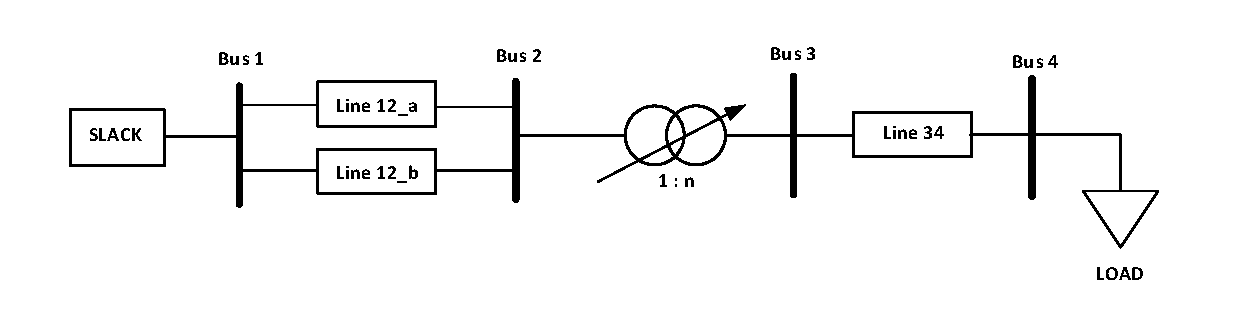
\includegraphics[width=0.9\textwidth]{PowerSystem_tap}
    \caption{Example Power System.}
\label{fig:pse1}
\end{figure}

The Automatic Voltage Regulator (AVR) logic of the tap-changing transformer is for low voltages, i.e., for increasing tap ratio. The model can be represented in the DSAR form as,


\begin{align*}
\dot{x_1}                   & =y_1y_7                                    \\
0                           & = y_2-V_3 + V_\text{low}                   \\
0                           & = y_3 - y_4 + z_1                          \\
0                           & = y_6 - n + n_\text{max} - n_\text{step}/2 \\
0                           & = nV_2-V_3                                 \\
0                           & = y_1 -1                   & y_2<0         \\
 \begin{matrix*}[r]
    0                                                                    \\0
  \end{matrix*}
                            &
\left.\begin{matrix*}[l]
= y_1                                                                    \\
= y_4-x_1
\end{matrix*}\quad\right\} & y_2>0                                      \\
0                           & = y_7 -1                   & y_6<0         \\
0                           & = y_7                      & y_6>0         \\
0                           & = y_5-x_1+z_1+T_\text{tap} & y_3<0         \\
0                           & = y_5-x_1+y_4+T_\text{tap} & y_3>0         \\
  \begin{matrix*}
    z_1^+                                                                \\  n^+
  \end{matrix*}
                            & \left.\begin{matrix*}[l]
= x_1^-                                                                  \\
= n^-+n_\text{step}
\end{matrix*}\quad\right\} & \text{when} \quad y_5=0
\end{align*}

The continuous dynamics of the real power load in bus 4 is given by

\begin{align*}
\dot{x_p} = \frac{1}{T_p} (P_s^0-P_d)\\
P_d = x_p + P_t V_4^2
\end{align*}

where, $x_p$ is the load state driving the actual load demand $P_d$. In response to voltage disturbance, the load undergoes an initial transient given by the term $P_t V_4^2$ and rate of recovery is dictated by the load time constant $T_p$.

\begin{table}[H]
  \caption{Base case parameters.}\label{tab:dataps}
  \centering
  \begin{tabular}{p{2cm}l}
    \toprule
    \emph{Component} & \emph{Parameters}                                                                                    \\
    \midrule
    Line 12\_a       & $R=0 \quad X = 0.65$                                                                                 \\
    Line 12\_b       & $R=0 \quad X = 0.40625$                                                                              \\
    Line 34          & $R=0 \quad X = 0.80$                                                                                 \\
                     &                                                                                                      \\
    Slack            & $|V|= 1.05 \quad \angle = 0^\circ$                                                                         \\
    Transformer      & $V_\text{low}=1.04 \quad n_\text{max} = 1.1 \quad T_\text{tap} = 20.0 \quad n_\text{step} = 0.0125 $ \\
    Load             & $P_s^0=0.4 \quad P_t = 0.4 \quad T_p = 5  $                                                          \\
    \bottomrule
  \end{tabular}
\end{table}
The data of the test system is given in Table \ref{tab:dataps}. The simulation is carried out by tripping the line (Line 12\_b) at 10s. The initial tap position is set to 1.0375. The simulation results are shown in Fig. \ref{fig:tps}.

\begin{figure}[H]
 \begin{subfigure}[b]{0.5\textwidth}
    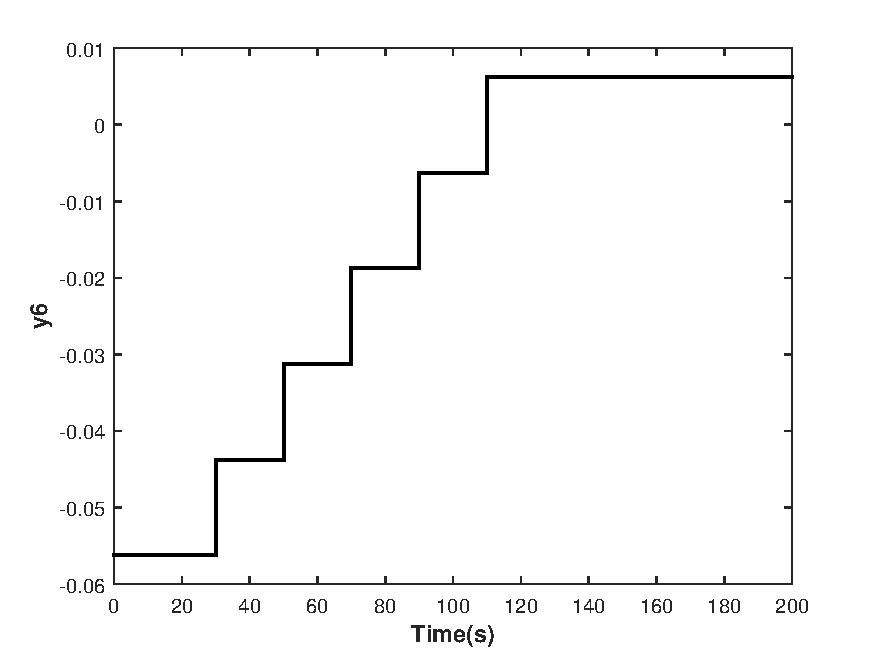
\includegraphics[width=\textwidth]{y6}
    \end{subfigure}
  \hfill
  \begin{subfigure}[b]{0.5\textwidth}
    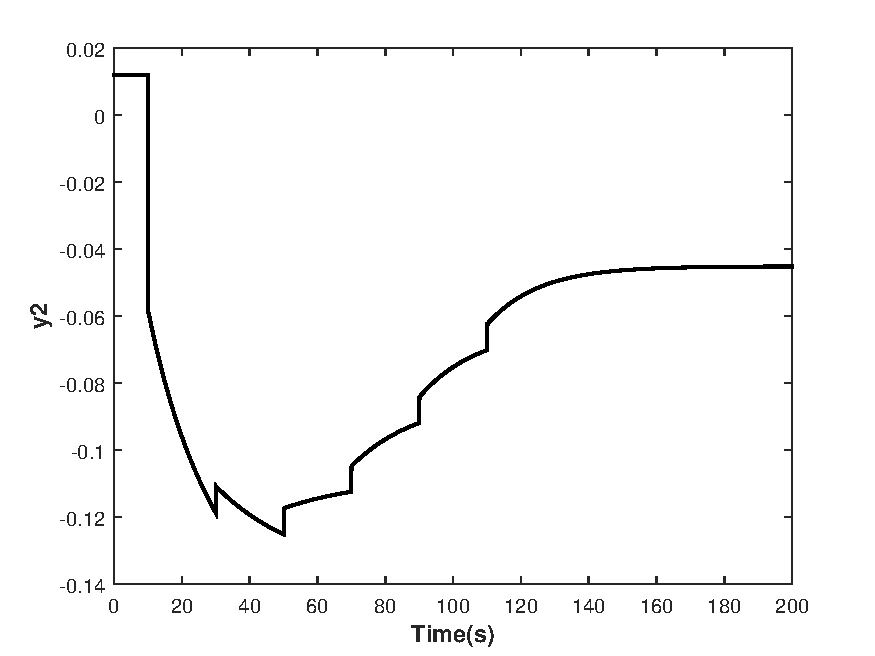
\includegraphics[width=\textwidth]{y2}
    \end{subfigure}
    \begin{subfigure}[b]{0.5\textwidth}
    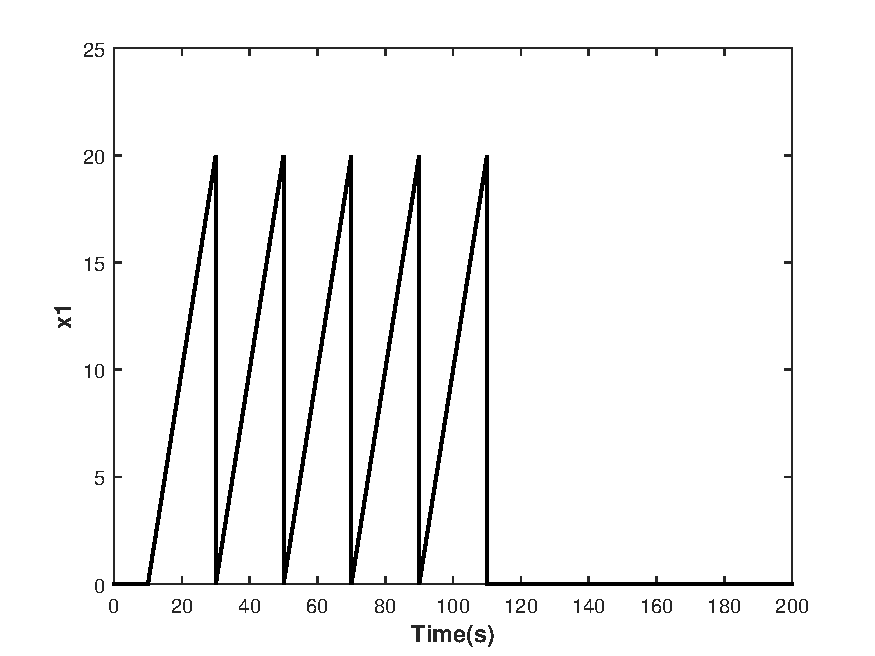
\includegraphics[width=\textwidth]{x1}
    \end{subfigure}
    \begin{subfigure}[b]{0.5\textwidth}
    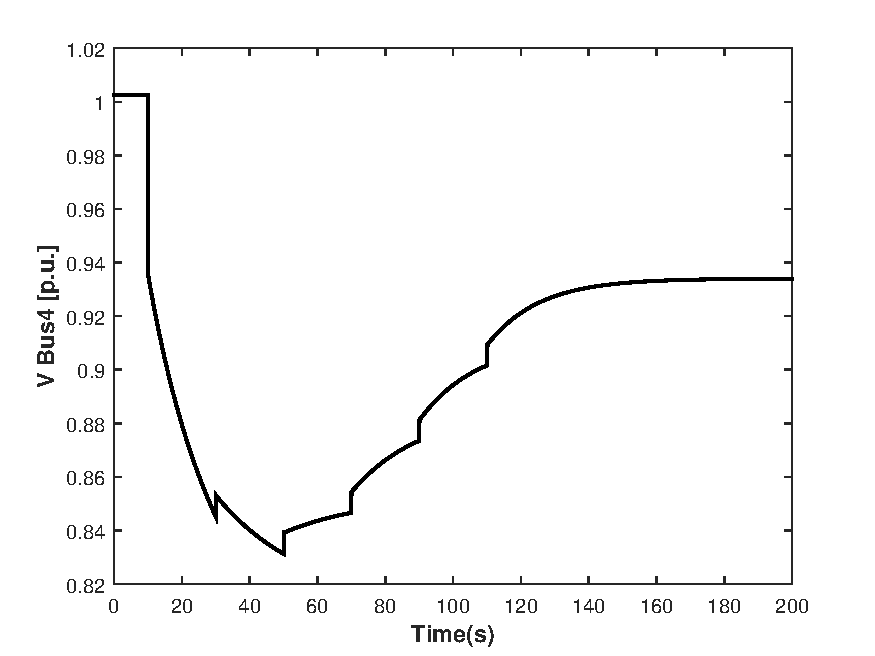
\includegraphics[width=\textwidth]{vbus4}
    \end{subfigure}
    \begin{subfigure}[b]{0.5\textwidth}
    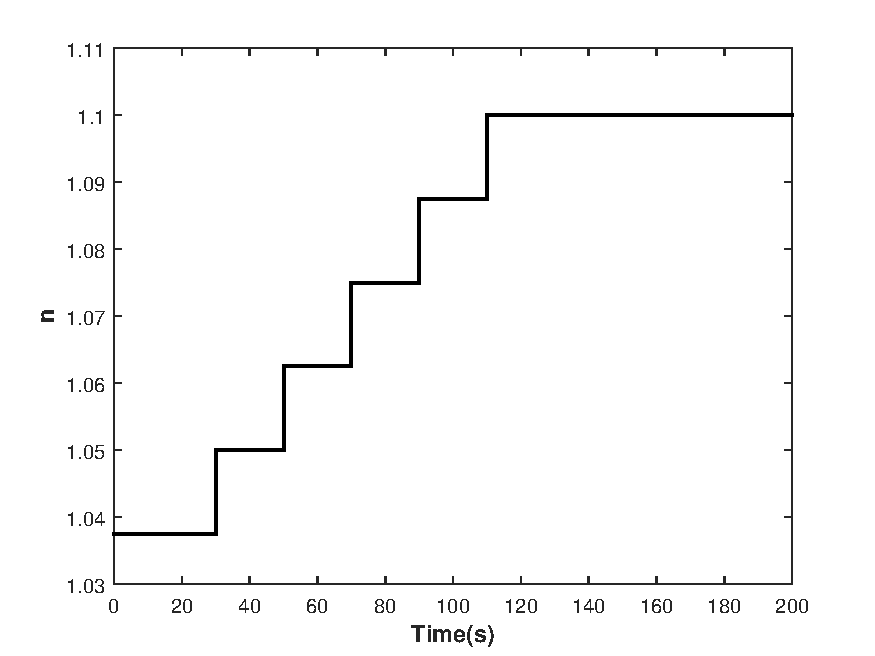
\includegraphics[width=\textwidth]{n}
    \end{subfigure}
    \begin{subfigure}[b]{0.5\textwidth}
    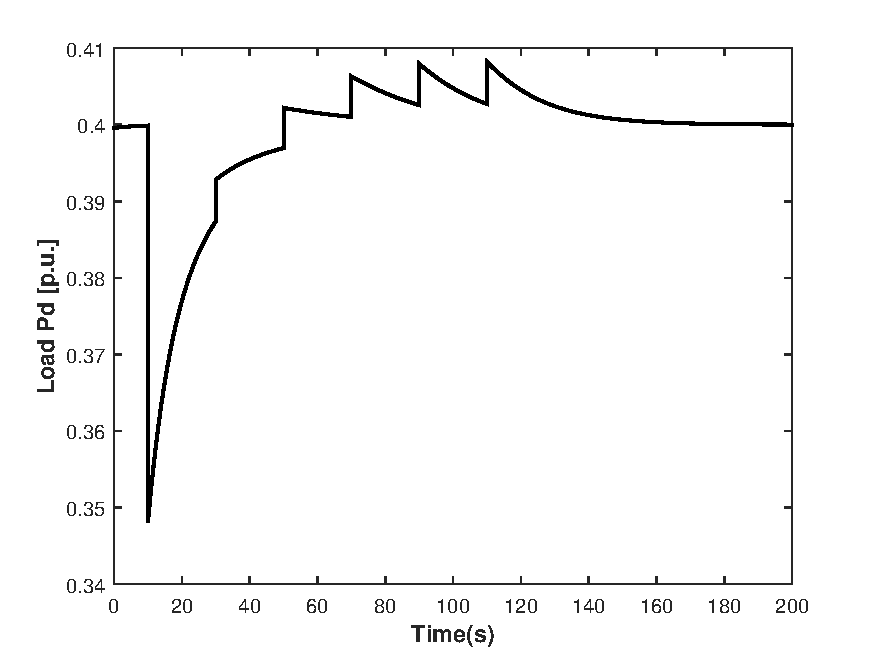
\includegraphics[width=\textwidth]{pd}
    \end{subfigure}
  \caption{Trajectories of Example power system.}
  \label{fig:tps}
\end{figure}

The dynamics of the tap-changing transformer are driven by different events that govern the behaviour of the timer. If the voltage is within the dead-band ($y_2<0$) or, the tap position is at the upper limit ($y_6>0$) then the timer is blocked. When the voltage is outside the dead-band ($y_2<0$), the timer will run and if the timer reaches $T_\text{tap} (y_5=0)$, a tap change will occur. After every tap change the timer will be reset, but not necessarily blocked. From the simulation results shown in Fig. \ref{fig:tps}, it is evident that the proposed DSAR structure with appropriate simulation framework is capable of simulating combined continuous and discrete dynamics of power systems.

\subsection{Extended version}

The updated model is: \texttt{TransformerDiscrete2}. This model considers the voltage deadband: [vlow vhigh] and the tap can go in both direction. Simulation is carried out by tripping the breaker of line (Line 12\_b) at 20s and re-closing the breaker at 200s. The trajectories of voltage at Bus 3 and tap ratio are shown in Fig. \ref{fig:updated}.

\begin{figure}[H]
\centering
 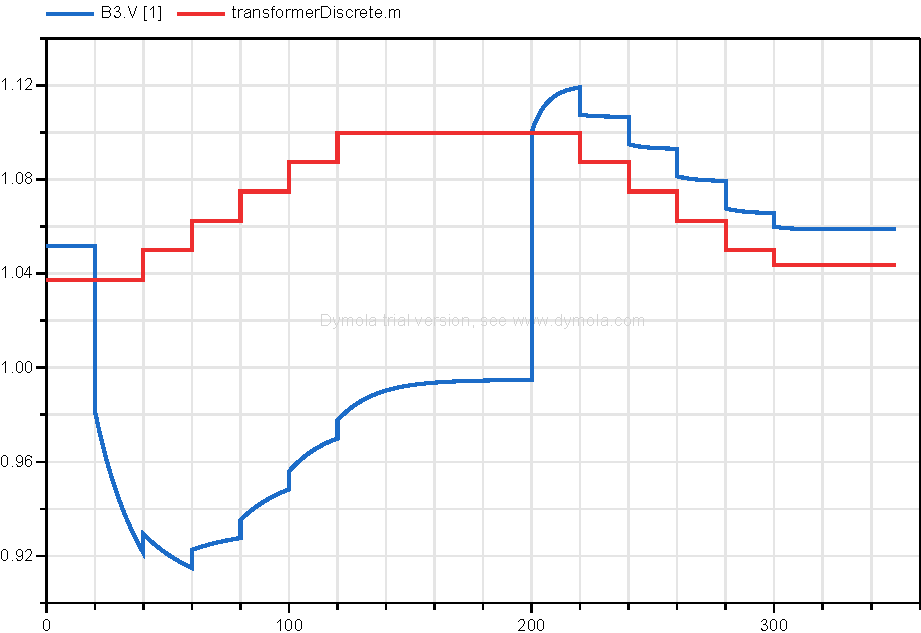
\includegraphics[width=0.8\textwidth]{vm}
    \caption{Trajectories of updated ULTC.}
\label{fig:updated}
\end{figure}

\bibliography{ultc}
\bibliographystyle{ieeetr}

\end{document}
